\documentclass[a4paper]{article}
\usepackage[utf8]{inputenc}
\usepackage[frenchb]{babel}
\usepackage[T1]{fontenc}
\usepackage{fullpage}
\usepackage{graphicx}
\usepackage{listings}

\title{Projet multicore programming}
\author{Thibault \bsc{Bèziers la Fosse}, Benjamin \bsc{Moreau}}
\date{28 Février 2016}

\begin{document}

\maketitle

\section{Introduction}
    \paragraph{}
    L'objectif de ce projet est d'implémenter une version parallélisée avec le langage \emph{C++} de l'algorithme de branch \& bound par intervalles afin d'encadrer le minimum d'une fonction de deux variables réelles.
    
    La parallélisation du code se fera en deux étapes. Dans un premier temps, nous utiliserons \emph{MPI} pour effectuer le calcul en coopération sur plusieurs machines. Dans un second temps, nous paralléliserons le code au sein de chaque machine à l'aide de \emph{OpenMP}. Dans chaque partie, nous justifierons nos choix d'implémentation et présenterons les résultats obtenus.
    
\section{Parallélisation avec \emph{MPI}}
    \subsection{Implémentation}
    \paragraph{}
    A l'aide de \emph{MPI}, nous avons décidé de paralléliser le programme au début de l’exécution. La boite contenant la fonction est coupée en $N$ sous-boites chacune prise en charges par les $N$ processus.
    Le premier processus demande à l'utilisateur la fonction à analyser puis \emph{broadcast} le choix à tout les autres. Il demande ensuite la précision à l'utilisateur et la \emph{broadcast} aux autres processus.
    Enfin, chacun appelle l'algorithme de \emph{Branch \& Bound} sur sa sous-boite calculée à l'aide du nombre de processus $N$ et de son rang $K$. Le minimum est trouvé en faisant un \emph{reduce} des minimums trouvés dans chaque sous-espace.
    \begin{center}
    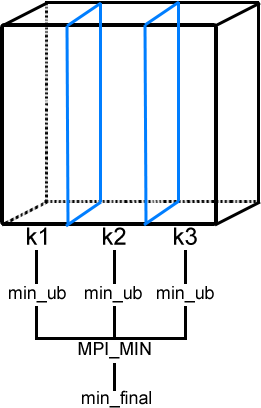
\includegraphics[scale=0.7]{min_mpi.png}
    {\footnotesize

    parallélisation MPI avec 3 processus (figure 1)\par}
    \end{center}
    \paragraph{}
    L’inconvénient de notre solution est qu'elle ne prend pas en compte la structure \emph{minimizer}. Pour régler ce problème, il faudrait que cette dernière soit partagée entre les processus \emph{MPI}. Chaque processus travail donc de façon indépendante sur son sous-espace. Cette parallélisation n'est pas efficace dans le cas ou les minimums possibles se retrouve rapidement dans un espace délimité par un des processus. Au contraire, Si la fonction est fluctuante, les minimums possibles seront distribués sur chaque processus ce qui augmentera son efficacité.
    \subsection{résultats}
    \paragraph{}
    
\section{Parallélisme à mémoire partagée avec \emph{OpenMP}}
	\paragraph{}
	Nous avons choisis \emph{OpenMP} pour la parallélisation à mémoire partagée car il très facile d'utilisation. De plus, l'utilisation de \emph{pragma} permet à l'utilisateur d'utiliser le code source sans forcement posséder la librairie \emph{OpenMP}. Malgré sa souplesse d'utilisation, il offre de bonnes performances.
    \subsection{Implémentation}
    \paragraph{}
    La parallélisation du code ce fait au sein de l'algorithme de \emph{Branch \& Bound}. Dans cette fonction, si la précision n'est pas suffisante, l'espace cubique contenant la fonction est coupé en 4 sous-espaces et la fonction est rappelée récursivement sur ces sous-boites. Nous parallélisons donc l'appelle récursif de cette fonction. A chaque appelle de la fonction, 4 exécutions parallèles de code sont donc lancés.
    
    Ces exécutions parallèles accèdent à une variable commune qu'il faut donc protéger : la liste de minimum courant. Nous utilisons donc un \emph{pragma} définissant une section critique à chaque fois que la variable est modifiée au sein de la fonction parallélisée.
    \subsection{résultats}
    \paragraph{}
    
\section{Conclusion}
    \paragraph{}
    Les résultats de nos jeux d'essais montre que la parallélisation à mémoire partagée permet d'augmenter l'efficacité de l'algorithme de façon significative. Sans les comparer, les résultats de l'exécution de l'algorithme à l'aide de MPI ne permet pas d'améliorer significativement l'efficacité de l'algorithme. En effet, Les processus travaillent séparément sans échanger leur minimums.
    
    L'idéal serait de doter notre solution MPI d'une fonction d’échange de minimum afin de faire collaborer les processus. Pour augmenter son efficacité, la parallélisation à mémoire partagée pourrait être ajoutée. Dans ce cas, la boite serait distribuée en fonction du nombre de machines. Puis, chaque ordinateur découperait l'exécution sur ses \emph{threads physiques} disponibles. Cette double parallélisation du code pourrait entraîner une amélioration importante du temps de calcul.
    
    

\end{document}